\documentclass{beamer}
\usepackage{ru}
\author[Flip \& Lars]{Flip van Spaendonck \& Lars Kuijpers}
\title{Compiler Construction \\ Barking up the wrong tree}
%\setbeamercovered{transparent} 
%\setbeamertemplate{navigation symbols}{} 
%\logo{} 
%\institute{} 
%\date{} 
%\subject{} 
\begin{document}

\begin{frame}
\titlepage
\end{frame}

\begin{frame}
\frametitle{Recap}
\begin{itemize}
\item Bottom-up parser
\item Separate Lexer and Parser
\item Written in Java
\end{itemize}
\end{frame}

\begin{frame}
\frametitle{Tree processing}
\begin{itemize}
\item Maps tokens to token traces
\item Combines all token traces into a tree
\end{itemize}
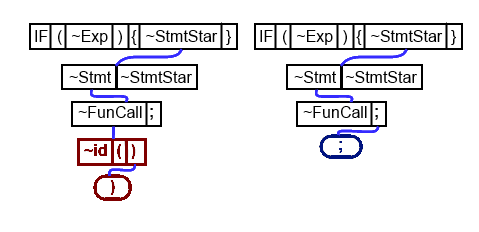
\includegraphics[scale=.5]{TokenTraces.png}\\
\pause
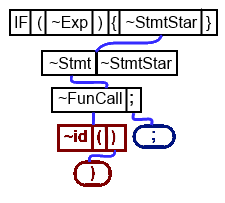
\includegraphics[scale=.5]{TokenTree.png}
\end{frame}

\begin{frame}
\frametitle{AST structure}
\begin{itemize}
\item Expressions can get a special identifier
\item Expressions with special identifiers are transformed in the tree
\item We identify the following expressions:
\begin{itemize}
\item Variable declaration
\item Variable assignments
\item Function declaration
\item Function calls
\item If-Else statements
\item While statements
\item Return statements
\end{itemize}
\end{itemize}
\end{frame}

\begin{frame}
\frametitle{Semantical Analysis}
Monomorphic Type Checking
\begin{itemize}
\item Check used IDs are well-defined
\item Check basic function types
\item Check defined function types
\item Check boolean conditions (if and while)
\end{itemize}
\end{frame}

\begin{frame}
\frametitle{Difficulties}
\begin{itemize}
\item Finalizing tree structure
\begin{itemize}
\item Made the type checking much easier
\end{itemize}
\end{itemize}
\end{frame}

\begin{frame}
\frametitle{Extensions}
\begin{itemize}
\item Structure makes it easier to add extensions
\item If you keep everything well-typed, currying works
\end{itemize}
\end{frame}

\begin{frame}
\begin{block}{Fun Metrics}
\begin{tabular}{l l}
\textbf{LOC} & 3616 \\
\textbf{Word count} & 9684 \\
\textbf{Character count} & 98470 \\
\textbf{Slides made} & 17 \\
\textbf{Coffee consumed} & 0\\
\textbf{Sanity lost} & A bunch \\
\textbf{Experience} & Priceless 
\end{tabular}
\end{block}
\end{frame}

\begin{frame}
\center{\Huge{Questions ?}}
\end{frame}

\end{document}